\chapter{Feature Engineering}
\label{chap:fea}

\todoA{FEATURE SELECTION FOR
KNOWLEDGE DISCOVERY AND
DATA MINING
Huan Liu
Hiroshi Motoda}


We cannot use the raw data for training as it is.
Instead, we represent each instance by a set of features;
each feature expressing a certain property of the instance.
An example of a feature can be the number of words in the review,
whether the~word {\it food} is present in the review
or a piece of metadata, like how many stars the user gave.

Features are of three types according to their values~---~nominal, ordinal and continuous.
Nominal features are discrete and there is no relationship between their values.
When a~feature is ordinal, it means it is discrete and also defines an ordering of the values.
Continuous feature is any real-valued variable.

In this thesis, we will utilize nominal and ordinal only.
We will omit the order in ordinal features and work with them the same way as nominal.
This of course loses information conveyed in this ordering,
but allows us easier feature manipulation.


\section{Extraction}

\textbf{Feature extraction} is the process of computing feature values for individual instances.
This may involve various operations on the given data.
Commonly used techniques include spell checking, converting geographic coordinates to names
or different linguistics analyses.

Also, it is often needed to split text into words.
Splitting text in general is called {\bf tokenization} and
the resulting units are called tokens (words in this context).
We use the nltk Tweet tokenizer\footnote{\url{https://www.nltk.org}}.
The tokenizer split words by spaces and punctuation.
It also considers punctuation marks to be tokens as well.
This allows the features to carry some potentially useful information.
An example is the indication that a word is at the end of a sentence when followed by a full stop.

Subsequently, it is often needed to convert words into lower case and {\it lemmatise} them.
Both these techniques help to group together words that express the same meaning.
{\bf Lemmatisation} is replacing a word with its lemma, which is a {\it base form} of the word.
The word \textit{cars} will be therefore be treated in the same way as \textit{car}.
Of course, the exact meaning of the two words is different,
but the fundamental idea is the same.
For the purposes of classification, it is often unnecessary to known whether there is one car or more.

For this analysis, we omit lemmatisation and use only lower case conversion.
Lemmatisation in English documents does not usually bring a big improvement,
because English is not a highly inflectional language.

\section{Selection}

Machine learning is used in contexts where the inner logic of~data is unknown.
It is therefore difficult to come up with useful features.
A common approach is to extract as many features as we can hoping some of them will be useful.
Because having too many features can lead to undesirable effects,
several techniques have been introduced to reduce the number of features
while retaining as much information about the class labels as possible.

Having fewer features which are informative enough leads to three direct benefits.
First, the resulting model is far less complex and as~such easier to~interpret.
Second, The~model also generalises better, because the~risk of overfitting is lower.
Overfitting happens when the~model recognises irregularities in training data
and learns to recognise individual instances.
It should instead approximate the~general concept to~be able to~classify new instances.
Lastly, fewer features result in shorter training time.

Three methods of feature selection are generally recognised; filters, wrappers and embedded methods.

\subsection{Filters}
\label{subsec:filters}

Filters work with individual features independently of any supervised classification algorithm.
The main objective of filters is to filter out features that are not informative on their own.
They evaluate the \textit{informativness} of each feature individually
and drop all bellow a certain threshold.

Filters are popular, because their time complexity is linear in the~number of~features.
However, the feature selection may~not be optimal,
because neither the~used classifier nor feature correlation is taken into account.

Such a~case is documented by \citet{GuyEli03} in \autoref{fig:guyeli03-figure3}.
The bottom left graph shows the original data and the~top left shows projection onto only one axis.
It is clear that one variable cannot be sufficient for separating the clusters.
However, if we project the data onto a combination of the two axes,
the clusters can be at least partially separated as can be seen in the right part of the figure.
Even though the solution to partially separate the two clusters exist,
no filter will choose either feature, because individually they are useless.

Another example of non-optimality is
features such that any single feature is individually sufficient to separate the data.
Optimal solution is  to choose just one of them.
However, any filter will choose all of them, because separately they are all useful.
This problem can be partially solved by the advanced method described in \autoref{subsubsec:mi}.
However, it increases the time complexity, which is the biggest advantage of filters.

%reverse example
%Suppose there are highly correlated features,
%each individually begin very informative.
%Because they are correlated,
%the information conveyed in some may be inferred from others.
%As a result, it is unnecessary to choose all of them.
%However, any filter will choose all of them,
%because filters consider features independently of each other.
 
 \todoA{citation and vector}

\begin{figure}[ht]\centering
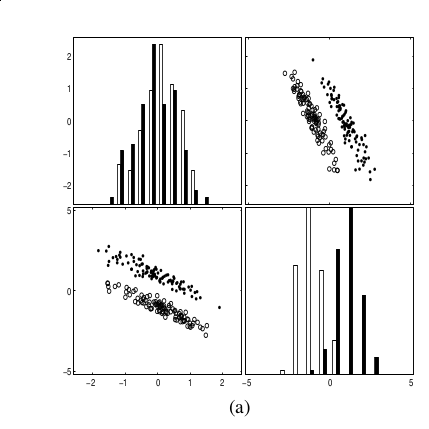
\includegraphics[width=100mm]{../img/guyeli_figure3.png}
\caption{Example of correlated features from the article}
\label{fig:guyeli03-figure3}
\end{figure}

There are number of filters differing in the filter condition.
We will discuss mutual information and Chi-square.

\subsubsection{Mutual Information}
\label{subsubsec:mi}
As \citet{Hoq14} defines it,
{\bf mutual information}~$I(X, Y)$~is the amount of uncertainty in X due to the amount of knowledge of Y.
{\bf Mutual information} of variables $X$ and $Y$ is defined as:

\begin{equation}
I(X,Y) = \sum_{x,y} p\left(x,y\right)
\log
\frac{p\left(x,y\right)}{p\left(x\right)p\left(y\right)},
\end{equation}

where $p\left(x, y\right)$ is the joint probability of~$X$ and $Y$ and~$p(x)$~and~$p(y)$~
are marginal probability distributions of the individual variables.

Mutual information can be also expressed as

$$I(X, Y) = H(X) - H(X|Y),$$

\todoB{explain entropy}

where~$H(X)$~is the entropy of~$X$~and~$H(X|Y)$~the conditional entropy.
This way~$H(X)$~expresses the amount of uncertainty of~$X$~and~$H(X|Y)$~what~$Y$~does not say about~$X$.
This supports the intuitive idea that information gain expresses how much information one variable carries about the other one.

The basic approach for selecting features is
to compute mutual information of each feature and the class label.
Only features exceeding some given threshold are used for training.

There is also an improved algorithm proposed by \citet{Hoq14}.
Instead of choosing all features in one step,
only one feature is chosen is chosen any time.
We have two sets; selected ($S$) and candidates ($C$) features.
In the beginning, all features are in $C$.

Every step, we choose one feature from~$C$ and move it to~$S$.
Which feature is chosen depends on two values calculated for each feature from~$C$.
First, feature-class as in the basic approach.
Second, the average of mutual information between the feature and all features from $S$.
We choose such a feature that has the highest feature-class and also lowest average of feature-feature.
This prevents including highly correlated features in~$S$.

Let us demonstrate it on two correlated features~$A$~and~$B$.
Adding~$A$ into~$S$ results in~$B$ having higher average of mutual information with features from $S$.
As such, $B$ is less likely selected in the next steps.

We stop, once the mutual information of the feature chosen from $C$ and the class drops bellow a certain
threshold.
At the end, features from~$S$ are used for classification.
We have not used this approach due to the lack of time and used the basic approach only.


\todoB{example}

\subsubsection{Chi-square~---~$\chi^2$}

Chi-square test of independence can be thought of
as a measure of lack of the independence between two variables.
As in mutual information,
we will compute a special value for each pair feature-class
and based on some threshold we will choose the most informative features.
We will briefly discuss the idea and present an example.
More detailed description can be found in~\citet{Hugh13}.


Let us demonstrate this with an example.
We have instances of our reviews and we want to test how well
feature \textit{credit card} describes
labels \textit{useful} and \textit{not-useful}.
The feature expresses whether the phrase ``credit card'' is present in the text of a review.
To asses this, we want to compute~$\chi^2$ of the variables~$X$~and~$Y$.
First, representing the feature \textit{credit card}.
Second, the true label.

\autoref{tab:chi_ex} shows example data.
The inner cells express how many instances there are with the given combination of variable values.
The bottom most row and right most column express marginal probability distributions
calculated by the number of samples.
If the variables were truly independent,
we would expect the cells to be 15 and 35 in the first and second row, respectively.
We will introduce a cost function to reflect this
and~$\chi^2$~of the two variables will then be sum of the cost function over all cells.


\todoA{aligning and crop excess vertical lines}
\begin{table}[h!]
 \center
 \begin{tabular}{|l|l|c|c|c}
 \cline{3-4}
        &       & \multicolumn{2}{c|}{label} & \\
        \cline{3-4}
        &       & yes        & no            & $P_Y$ \\
        \cline{1-4}
 credit & yes   & 25         & 5             & 0.30 \\
        \cline{2-4}
 card   & no    & 45         & 25            & 0.70 \\
        \cline{1-4}
        & $P_X$ & 0.50       & 0.50          & 1
 
 \end{tabular}
 \caption{$\chi^2$~Example}
 \label{tab:chi_ex}
\end{table}

Let us have two random variables~$X$~and~$Y$.
Let us define~$O_{x,y}$ and~$E_{x,y}$
as respectively the number of observed and expected instances for~$X=x$~and~$Y=y$.
The value of~$O_{x,y}$~is simply the number of instances.
The value of~$E_{x,y}$ is computed from marginal probabilities.
Namely:

\begin{equation}
E_{x,y} = P_X(X=x) \times P_Y(Y=y) \times n,
\end{equation}

where~$P_X$~and~$P_Y$~are the marginal probabilities of the variables~$X$~and~$Y$
and~$n$~number of all instances.

We define $\chi^2$~of two random variables~$X$~and~$Y$~as:

$$\sum_{x \in X, y \in Y}{\chi^2_{y,x}},$$

where~${\chi^2_{y,x}}$ is $\left(O_{x,y} - E_{x,y} \right)^ 2 / E_{x,y}$.

This corresponds to our intuition.
If the variables are correlated,
the observed values will differ from expected and~$\chi^2$ will by non-zero.
The farther observed value from the expected is, the higher penalization with square.
Also, it is normalized by dividing it in E.

The value of $\chi$ in our example in \autoref{tab:chi_ex}
~is:

\begin{equation}
\chi^2 = 
\frac{\left(25-15\right)^2}{15} +
\frac{\left(5-15\right)^2}{15} +
\frac{\left(45-35\right)^2}{35} +
\frac{\left(25-35\right)^2}{35}
\end{equation}

\begin{equation}
\chi^2 \approx 11
\end{equation}


\todoB{advantages/dis... a bit of discussion}

\subsection{Wrappers}

Unlike filters, wrappers work with subsets of features
and use a classifier to directly asses informativness of the subset as a whole.
Every subset is classified by the classifier used as a black box
and evaluated by some common evaluation metrics.
The optimal subset is than chosen.
Thanks to this, wrappers are universal and robust.

Furthermore, wrappers can perform a lot better than filters on certain datasets.
Such an example was shown in \autoref{subsec:filters}.

Unfortunately, wrappers tend to be computationally expensive,
because every subset must by classified separately.
In fact, it has been shown it is NP-hard to find optimal solution.
To achieve computational feasibility, various approximation methods has been developed.
These methods allow us to classify only a fraction of subsets
at the cost of losing the guarantee of the optimal solution.
We will describe two variants of greedy search.

\todoB{On the approximability of minimizing nonzero variables
or unsatisfied relations in linear systems --- citation of the NP-hard, otherwise delete} 

\subsubsection{Greedy Search --- Forward Selection}

{\it Forward selection} starts with an empty set and in every step adds a feature which brings the highest increase of performance in the evaluation metrics.
As we said, we use a classifier and some common evaluation metrics to asses the performance.
The score of a candidate feature is then difference between the performance of the classifier trained on the current feature set with this feature and without it.
The feature with highest score is added and the process repeated until the increase in performance is less than a certain threshold. 

\subsubsection{Greedy Search --- Backward Elimination}

{\it Backward elimination} works analogously to forward selection.
We start with the set of all features.
In one step a feature with lowest decrease in score is removed.
This step is repeated until the evaluation drops by more than a given threshold.
This approach may be infeasible for really big data sets, but guarantees to include all useful features of which some may be omitted by forward selection.

\subsection{Embedded Methods}

Embedded methods are part of a classification algorithm itself.
An example can be a decision tree, which takes features that lower the entropy the most first.
More on this in descriptions of particular algorithms.

\todoA{The last sentence should be removed if there are no such algos in this doc.}

\section{Principal Component Analysis}

Principal component analysis is not feature extraction nor selection.
It is rather an intermediate process between feature engineering and training a classifier.

\textbf{Principal component analysis} (PCA) is another way of reducing the number of features used.
Instead of selecting a feature subset, it treats instances as feature vectors.
A \textbf{Feature vector} is a vector wherein each element corresponds to a value of one feature.
The order of features is fixed.
This way we can represent an instance with all its features by a vector.

The idea of PCA is to transform feature vectors into a space of lower dimensionality.
The objective is to retain as much information contained in the vector, while
having lower dimensionality.
Mathematically speaking, the objective is to retain as much variation of variables
as possible and reduce any variable correlation.
The exact description is way beyond the scope of this text.
More detauled explanations can be found in~\citet{Jolliffe02}.

\section{Commonly Used Features}

In this section, we will use some commonly used features and briefly discuss their pros and cons.

\subsection{Bag-Of-Words}
\label{subsec:bow}

Since the information a sentence carries is not contained only in the words, but also in their positions in the sentence, an ideal algorithm would take into account both the words and their positions.
However, working with sentences as a whole is somewhat difficult. Hence, the order of words is often omitted and only the word occurrences matters.
\textbf{Bag-Of-Words} (BOW) encodes this information by mapping every word onto the number of occurrences in the given text.

\subsubsection{TF-IDF}

In a general document there are many words that are not directly useful.
{\it TF--IDF} is a way to evaluate which words are the most important for individual documents and
choose reduce the number of words used in BOW.
\citet{SalBuc88} describe the motivation for introducing this.
The goal is to select such words for a document
that they will define it well enough, yet leave enough room for describing all relevant documents by the same words.
We will introduce two metrics to convey these two requirements and then use a combination of those two to gain the best results.

First, we will simply use only words occurring frequently enough in a document.
The number of occurrences of a word in a document is referred to as {\it term-frequency}.
Second, we will use {\it inverse-document frequency} (IDF) to skip words such as {\it an}, {\it the} which appear in virtually every sentence and carry very little information.
IDF is indirectly proportional to the number of documents which contain a given word.
Thanks to this, words like articles will be given very little weight.

There are many implementations of this general idea.
We will explore the implementation described in \citet{Ramos03}.
Given a set of documents~$D$
we can calculate TF-IDF for word~$w$ in an individual document~$d$ as:

\[
	w_d = TF \times IDF = f_{w, d} \times \log \left( \frac{\abs{D}}{f_{w,D}}  \right),
\]

where $TF = f_{w, d}$ is the number of times~$w$~occured~$d$ and
IDF corresponds to $\log \left( \frac{\abs{D}}{f_{w,D}}  \right)$ for $\abs{D}$ being the total number of documents and $f_{w, D}$ the number of documents containing~$w$.

Let us explore how the value changes with different variable values.
For such words that $\abs{D} \sim f_{w, D}$ the value of logarithm is very low and so is the importance of the words.
This is desired behaviour because words that occur in virtually every document  are not very useful.
On the other hand, words having $f_{w,d}$ large and $f_{w,D}$ small are given much higher importance.
This is again desired, because these words occur relatively often in the given document and not so often in the document set overall.

\todoA{Is this really the way we're going to use it? We have very short texts}

\todoA{- TD*IDF - with given threshholds - how to find it?}

\todoB{try TD*IDF not with a~given threshold, but rather find te optimal threshold for cuts}

\subsection{N-grams}

When using BOW, we can potentially loose useful information conveyed in the word order.
Unfortunately, it is often computationally infeasible to retain the complete order.
To find a balance, N-grams try to convey the order only partially.
\textbf{N-gram} is simply a sequence of items, in our case words. The~$N$~refers to the length of the sequence.
The longer a sequence is the more order is preserved at higher computational cost.
Bigrams and trigrams (pairs and triples) are most commonly used.

\todoB{- choose words with highest information gain; as in McCallum Event models}

\subsection{Word Embeddings}
\label{subsec:wordembed}

Word embeddings is another way to convert words into features.
\citet{LeGo14} describe {\bf word embedding} as a mapping of every word to a vector in~$R^d$.
This is also sometimes referred to as \textit{distributed word representation}.
This mapping is obtained by using a big corpus of data and optimizing some cost function on it.

\citet{Mik13} showed that if parameters are set carefully, word embeddings conveys both semantic and sytanctic information.
First, similar words are mapped to similar vectors. So we can measure a sort of synonymity.
Not only that, but it also conveys relationships between words.
An example is singular vs plural.
Let~$x_{w}$ be the vector of the word~$w$.
They showed that $x_{apple}-x_{apples} \sim x_{car}-x_{cars}$.
Even more complicated relations like $x_{king} - x_{man} + x_{woman} \sim x_{queen}$ were shown.
They use this property to solve word analogies in the form {\it a is to b as c is to \_\_\_}.


\subsection{Geneea entities}http://aspell.net/

\bf entities extracted from geneea \rm

 \todoB{- filter them based on the~geneea value of importance}

 \todoA{- occurrences - pick only the~most frequent}

\subsection{\todoB{Cosine sim}}


\subsection{Hand Crafted Features}

\subsubsection{Spell check}

We also tried to measure typos in the review.
The hypothesis was that reviews with many typos may be less useful,
because the reviewer apparently did not spend much time writing it.
We used the open source package aspell \footnote{\url{http://aspell.net/}}
to compute the ratio of incorrect words out of all words.
Subsequently, we clustered the values into two groups; with and without typos.
We allowed instances with up to a few typos to be in the latter group.

\todoA{incoherent with appendix}

\subsubsection{Review length}

Another hand crafted feature was a review length.
It is simply the number of words as returned by the already described twitter tokenizer.
Again, we clustered values into groups to get binary or ternary features.


\subsection{non-textual features --- metadata}

Sometimes it may be necessary to use metadata
if the text itself does not contain enough information.
The exact usage will depend on the task.
We used metadata mostly for filtering out restaraunts without enough data.
The only feature we tried to extract from metadata was the number of stars the review gives.
We tested two approaches.
First, a simple feature expressing how many stars were given.
Second, we tried to have a feature \textit{extreme stars}.
This feature is binary being one if the user gave 1 or 5 stars;
zero otherwise.

We were hoping that reviews with 1 or 5 stars may express very strong opinion
and as such are more likely to be useful.

